\begin{frame}[t]{Orientácia}
\begin{itemize}
  \item<1-> riadenie orientácie, tj. uhly $\Omega={\Phi, \Theta, \Sigma}$ a uhlové rýchlosti $\dot\Omega$ v lokálnych súradniciach telesa \angl{body frame}
  \item<2-> Pre RC dron by to aj stačilo s ``plynom''  \angl{throttle} $h\rightarrow\tau$ na ovládanie ťahu \angl{thrust} motorov \footnote{Síce rate-control je tiež možné \citep{Boland2015}!} \citep{Boland2015}
  \item<3-> Riadiť orientáciu \angl{attitude} len na základe zmeny uhl. rýchlosti \angl{rate} by bolo dosť neintuitívne, potrebujeme prepočítať $r_{\Theta} \rightarrow r_{\dot{\Theta}}$ \footnote{Naopak môžeme vynechať rate controller, ako v MATLAB/Simulink príklade}
      \item<4-> Táto slučka je často nazvaná ako stabilizačné riadenie \angl{stabilize} alebo orientačné riadenie \angl{attitude control} \footnote{predošlá je \angl{rate}}
      \item<5-> Nezabudnime na štvrtú kaskadovanú slučku: výška $\rightarrow$ rýchlosť zmeny výšky resp. vertikálna rýchlosť \angl{climb rate} $\rightarrow$ zrýchlenie $\rightarrow$ motor
\end{itemize}
\end{frame}


\begin{frame}[t]{Orientácia}
\begin{itemize}
  \item<1-> Tvárme sa, že poznáme žiadané orientácie (napr. RC), napr. klopenie $r_{\Theta}$ a chceme riadiť $y_{\Theta}$.  V skutočnosti riešené s kvaternióny aby sme obišli singularitu Eulerových uhlov pri odhade \citep{Erasmus2020}. Ak by sme priamo pilotovali RC, bol by to tzv. stabilizovaný letový mód \citep{Boland2015}.
  \item<2-> Riadenie orientácie môže byť riešené ďalšou, nadradenou regulačnou slučkou - hovoríme o tzv. kaskádnom riadení \angl{nested, cascaded}.
  \end{itemize}


    \begin{onlyenv}<1>
  \begin{figure}
\centering
  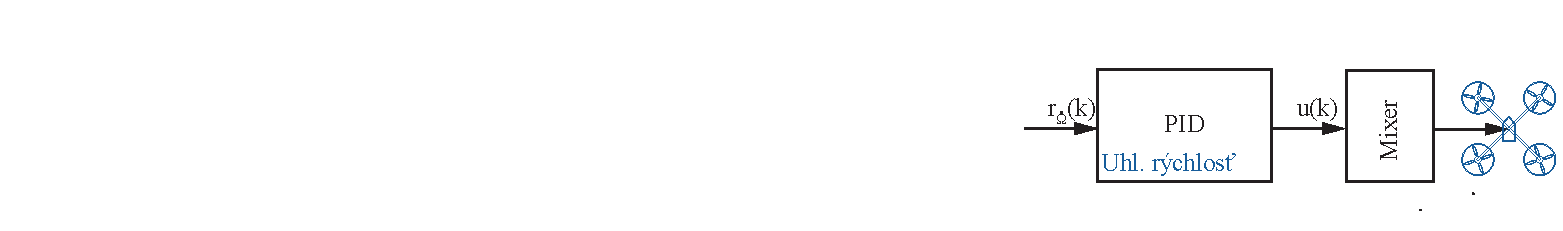
\includegraphics[width=\textwidth]{PID_HighLevel1a}\\
\end{figure}
\end{onlyenv}



    \begin{onlyenv}<2>
  \begin{figure}
\centering
  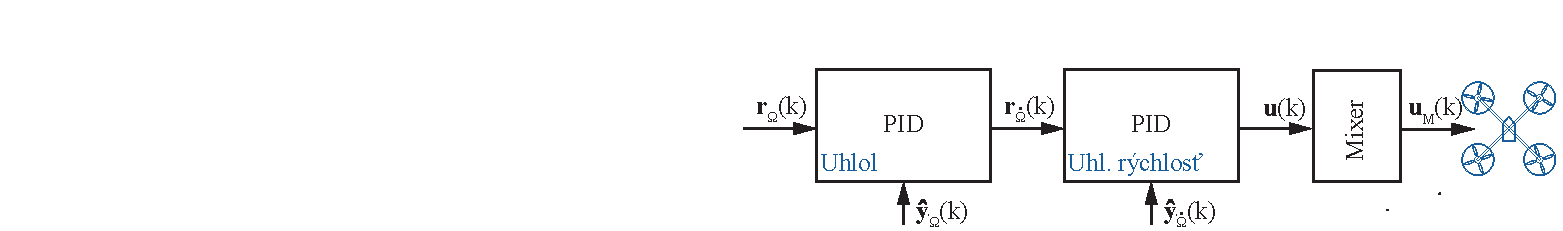
\includegraphics[width=\textwidth]{PID_HighLevel1b}\\
\end{figure}
\end{onlyenv}

  \end{frame}



\begin{frame}[t]{Orientácia 2}
\begin{itemize}
  \item<1-> Nadradené slučky sú pomalšie, vytvára to istý ``filter'', t.j. nemôžeme rýchlejšie ovládať rýchlosť ako polohu (cca. o rád, min polovicu pomalšie\footnote{ArduCopter 40 Hz vs 400 Hz, PX4 250 vs. 1000 Hz \citep{AP:PID,PX4:PID}}) \citep{AP:PID,PX4:PID}
  \item<2-> Pri PID skôr P\footnote{ArduCopter a PX4 Autopilot používa P regulátor \citep{PX4:PID,AP:PIDDOC}}, lebo D reaguje príliš agresívne na šum.
  \item<3-> Do slučky dopracujeme doprednú väzbu \angl{feedforward} ktorá zrýchli odozvu regulácie. ``Whatever works'' - netreba mystifikovať.
  \end{itemize}



  \begin{onlyenv}<2>
  \begin{figure}
\centering
  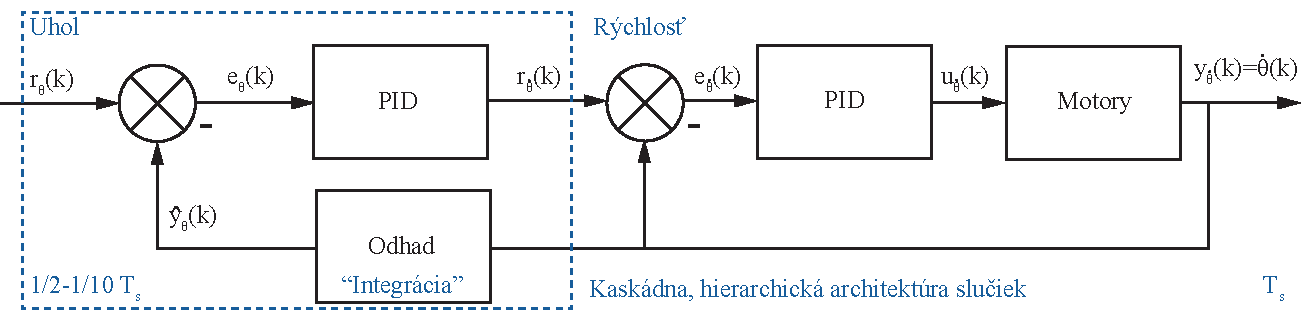
\includegraphics[width=\textwidth]{ATT_Angle}\\
\end{figure}
\end{onlyenv}

  \begin{onlyenv}<3->
\begin{figure}
\centering
  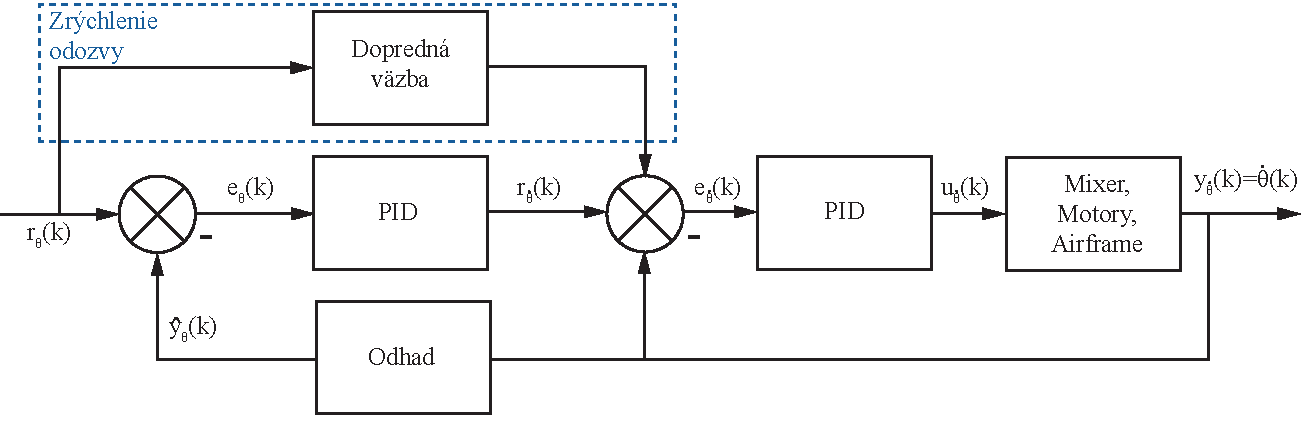
\includegraphics[width=\textwidth]{ATT_Angle2}\\
 \end{figure}
\end{onlyenv}

  \end{frame}

\begin{frame}[t]{Feeedforward}
\begin{itemize}
  \item<1-> Dopredná väzba - keď poznáme stálu časť akčného zásahu, prečo to rovno nepoužívať?
  \item<2-> Napr. pri stabilizácii letovej výšky máme $u_h=mg$ a zvyšok rieši regulátor
  \item<3-> Didaktický príklad v Simulinku uvažuje PD regulátor výšky + feedforward

  \end{itemize}



  \begin{onlyenv}<2>
  \begin{figure}
\centering
  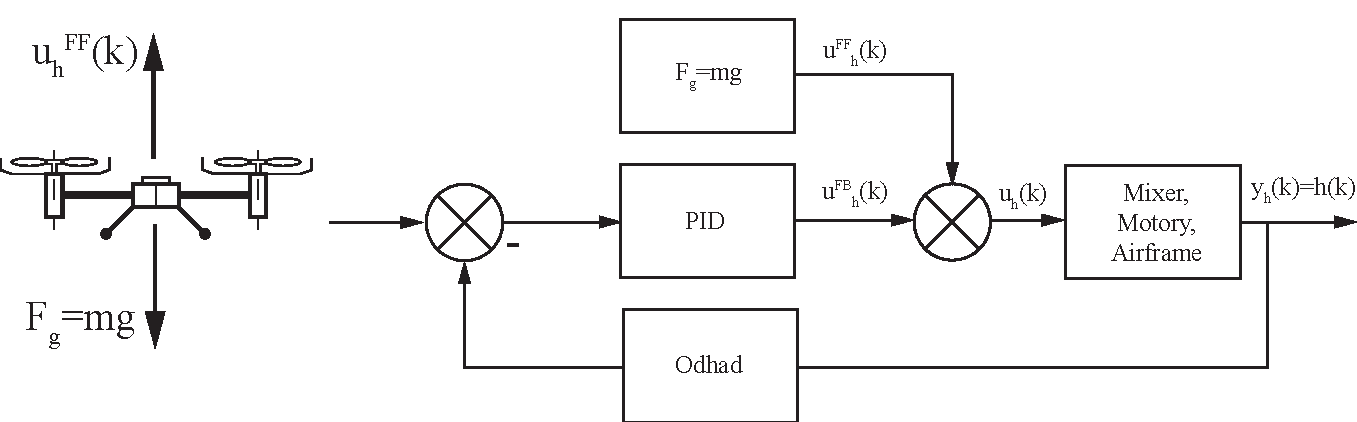
\includegraphics[width=\textwidth]{FF_Thrust}\\
\end{figure}
\end{onlyenv}

  \begin{onlyenv}<3>
\begin{figure}
\centering
  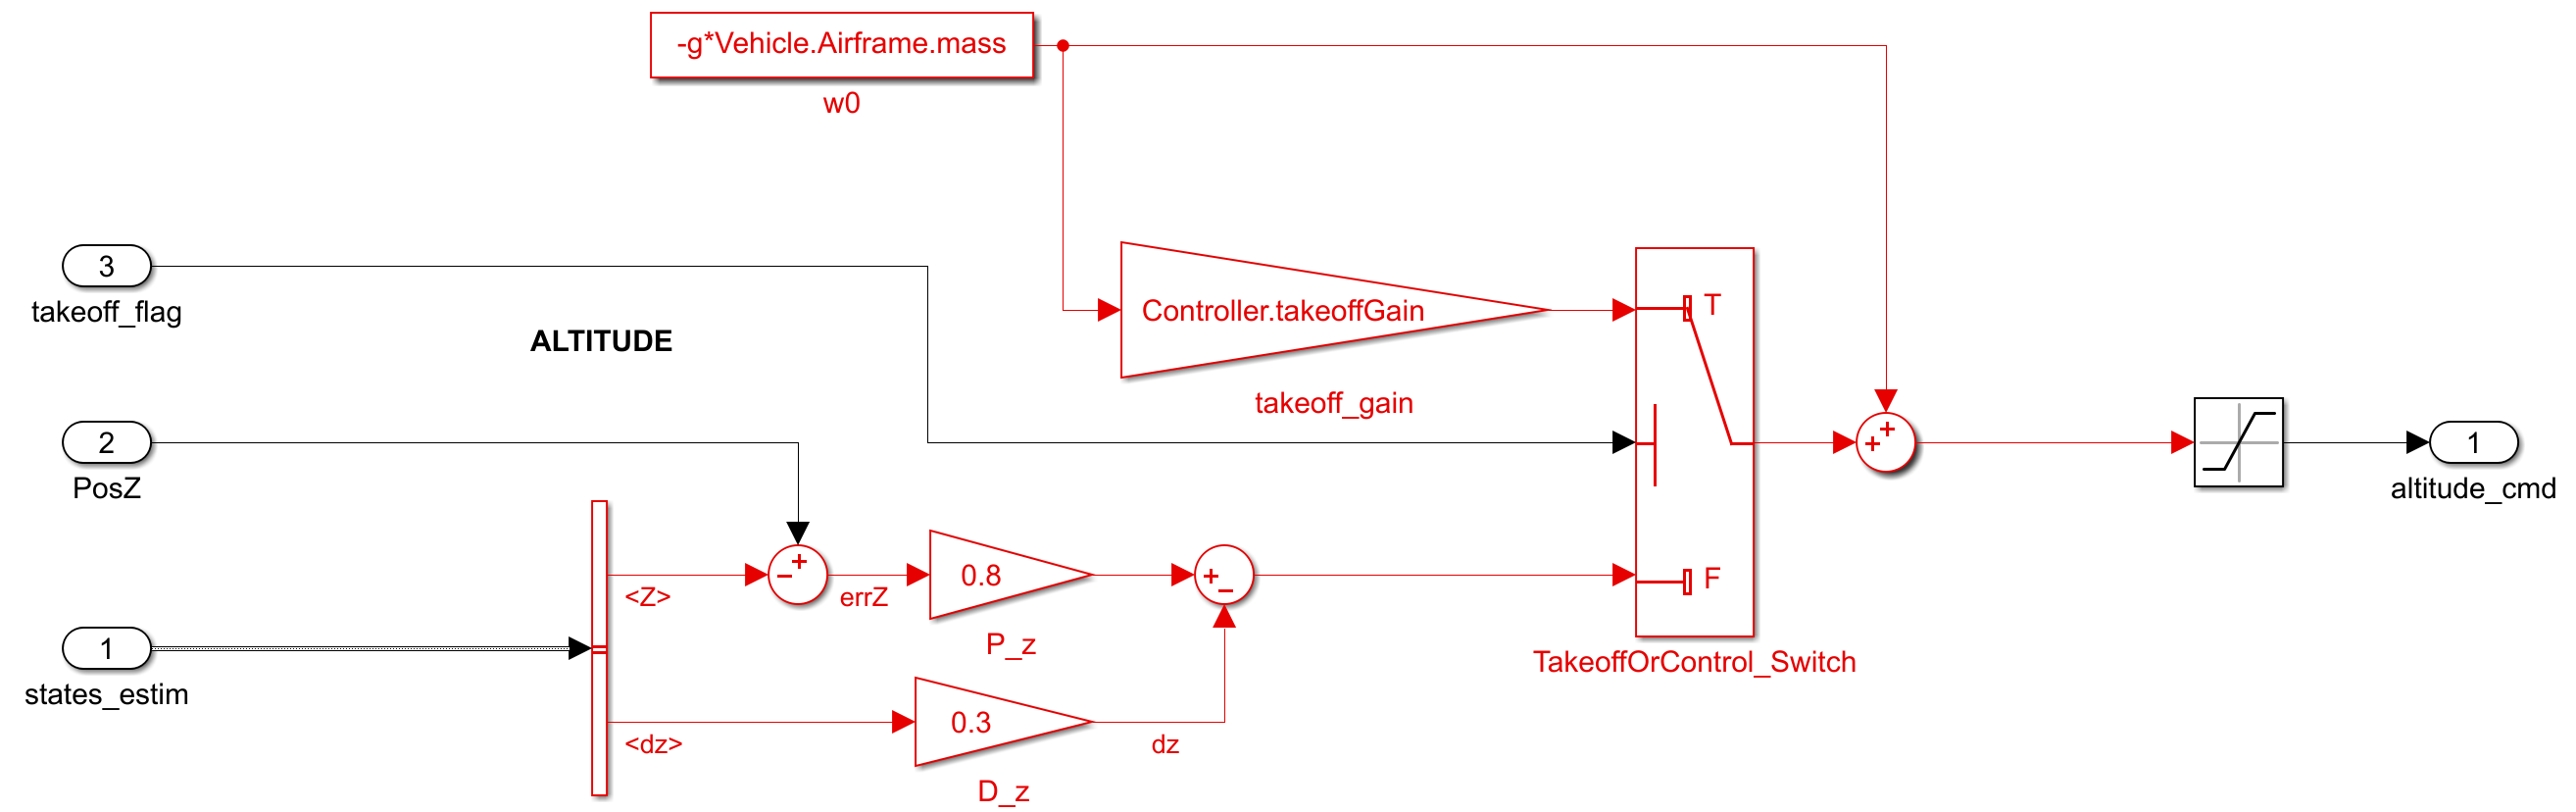
\includegraphics[width=\textwidth]{MS_FF}\\
 \end{figure}
\end{onlyenv}

  \end{frame}



  \begin{frame}[t]{Orientácia: PX4 a ArduCopter}
\begin{itemize}
  \item<1-> PX4 používa kvaternióny (pár slov o tom neskoršie), ale je to iba P regulátor
  \item<2-> ArduCopter v podstate taktiež tam má P regulátor + FF
\end{itemize}

  \begin{onlyenv}<1>
  \begin{figure}
\centering
  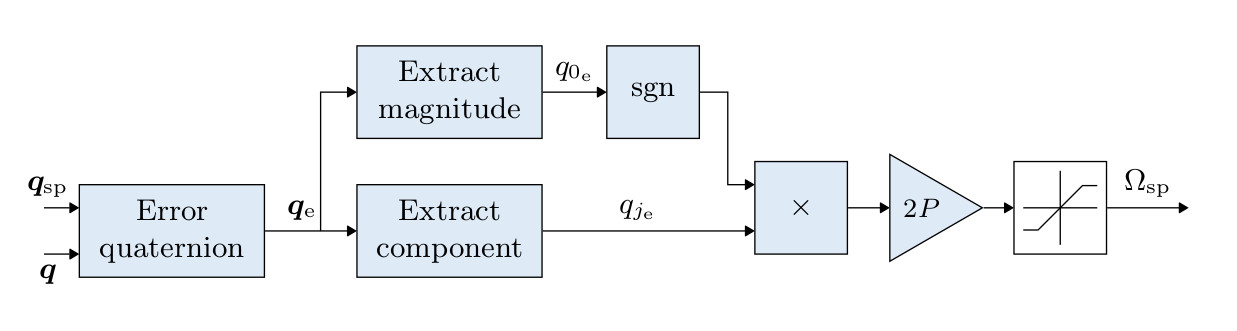
\includegraphics[width=100mm]{PX4_Angle}\\
\end{figure}
\end{onlyenv}


  \begin{onlyenv}<2>
  \begin{figure}
\centering
  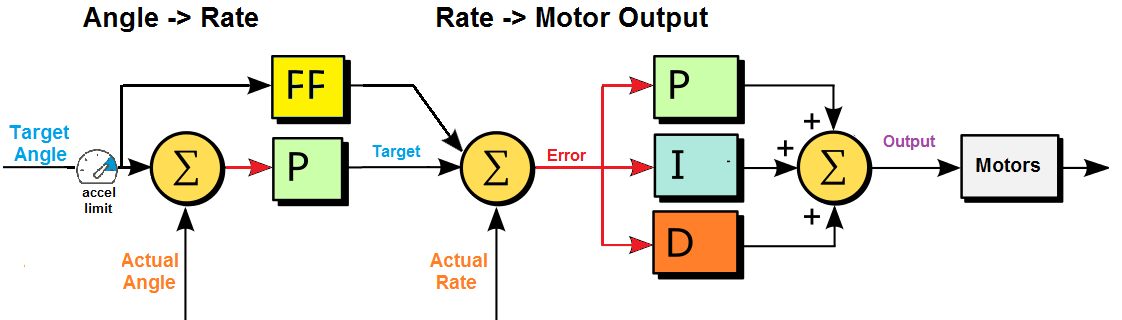
\includegraphics[width=80mm]{AP_Angle}\\
\end{figure}
\end{onlyenv}

  \begin{onlyenv}<3>
  \begin{figure}
\centering
  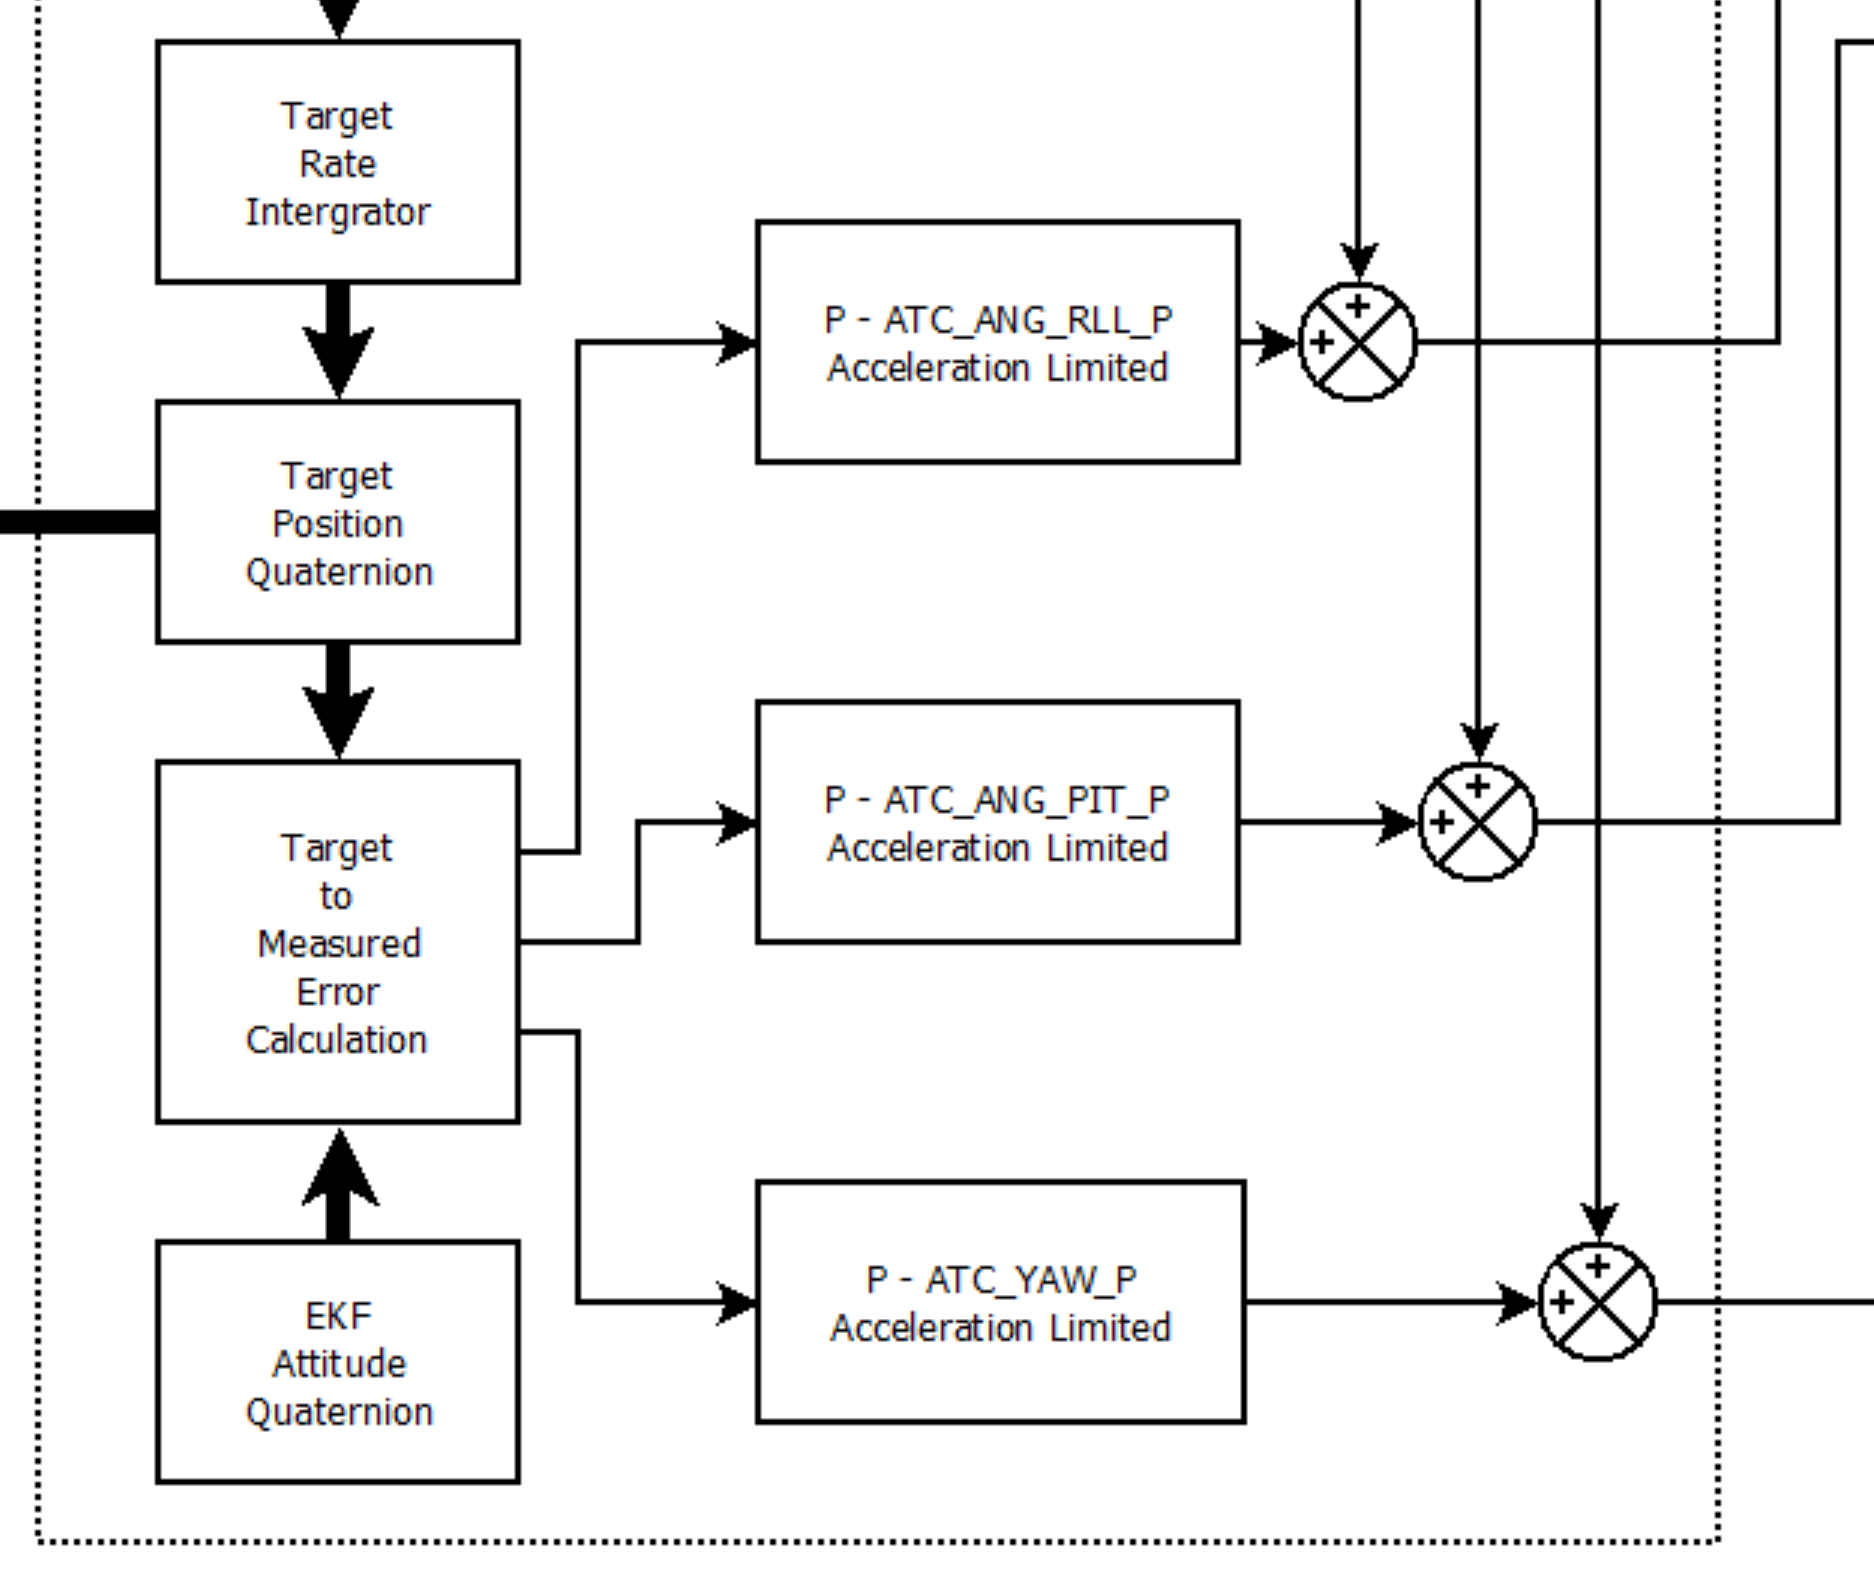
\includegraphics[width=80mm]{AP_Angle_New}\\
\end{figure}
\end{onlyenv}

  \end{frame}

\begin{frame}[t]{Orientácia: Problém stabilizácie}\
\begin{itemize}
  \item<1-> Máme 4 nezávislých slučiek
  \item<2-> Ako to vyzerá v MATLAB príklade?
  \item<3-> Čo sa stane ak chceme dron stabilizovať? Majme 0-vé Eulerove uhly!
  \item<4-> Určite to drží na jednom mieste?
  \item<5-> Potrebujeme nenulové klopenie a klonenie, a referenciu na základe polohy!
\end{itemize}
  \begin{onlyenv}<1>
\begin{figure}
\centering
  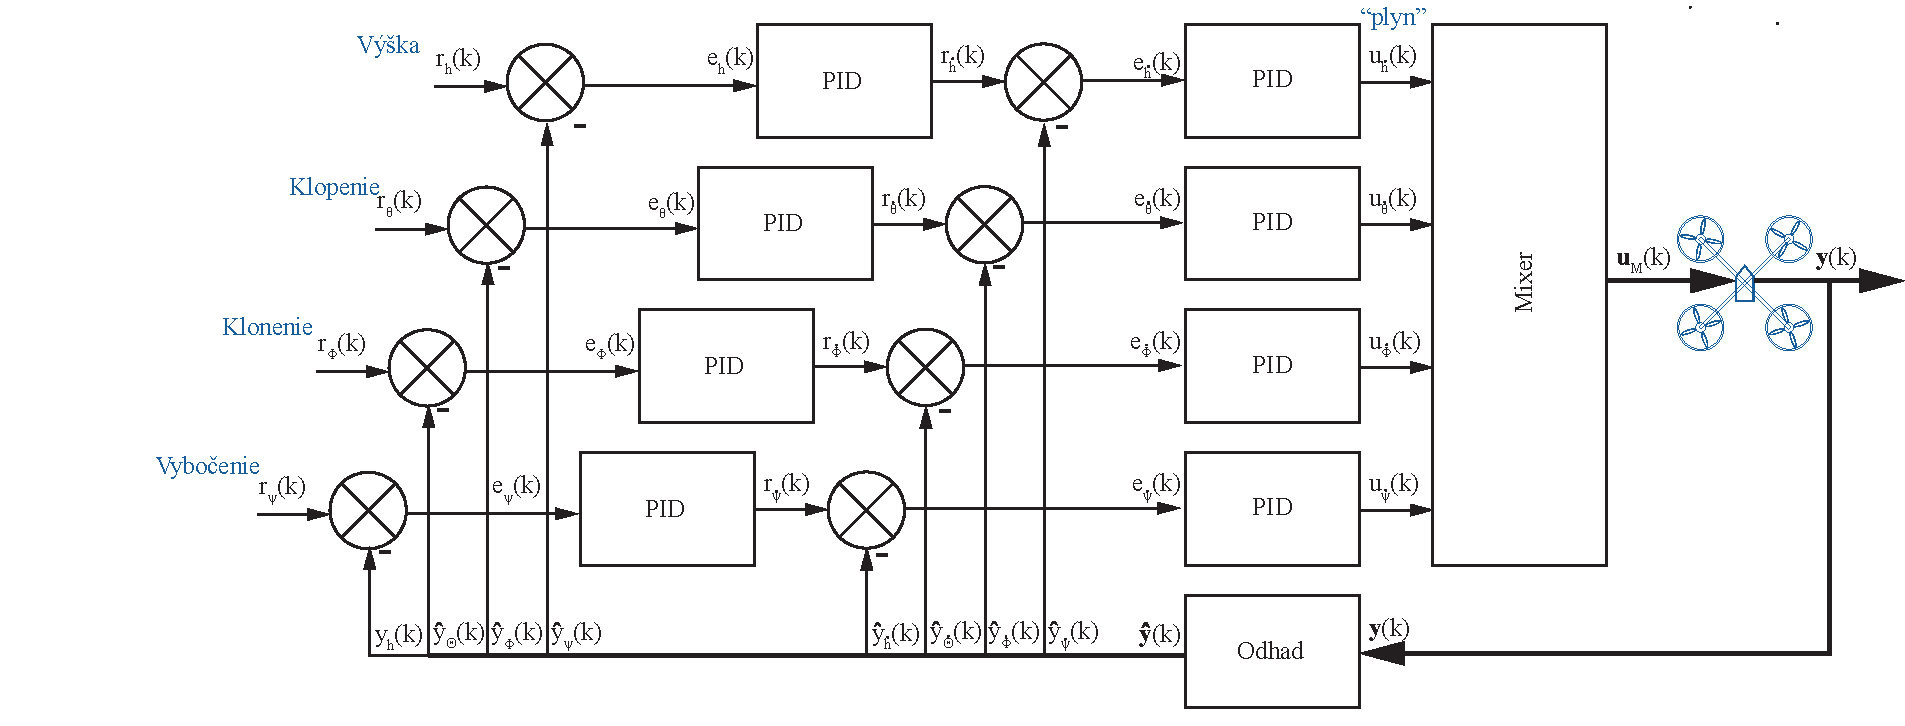
\includegraphics[width=\textwidth]{ATT_Overall1}\\
\end{figure}
  \end{onlyenv}

    \begin{onlyenv}<2>
\begin{figure}
\centering
  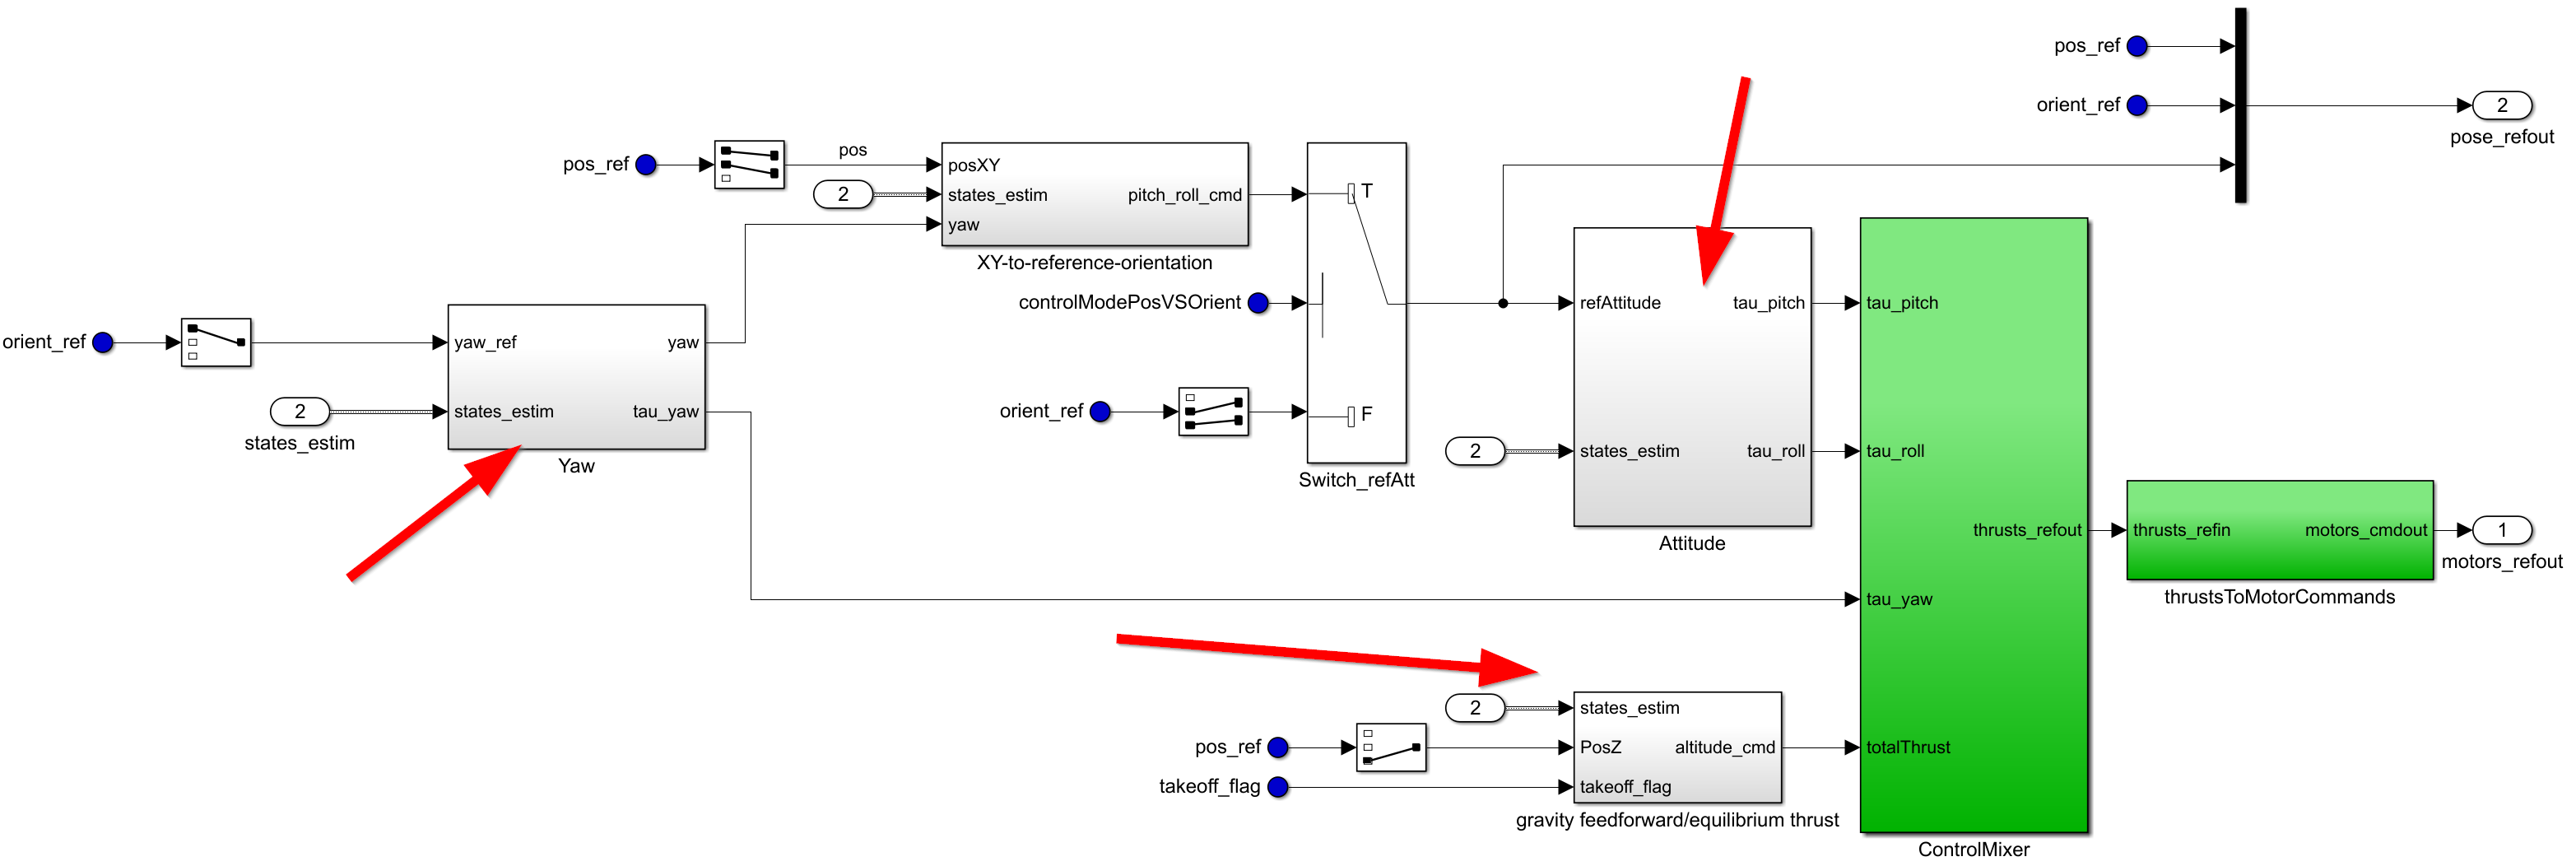
\includegraphics[width=\textwidth]{MS_QuadExample_AllRate}\\
\end{figure}
  \end{onlyenv}


    \begin{onlyenv}<3>
\begin{figure}
\centering
  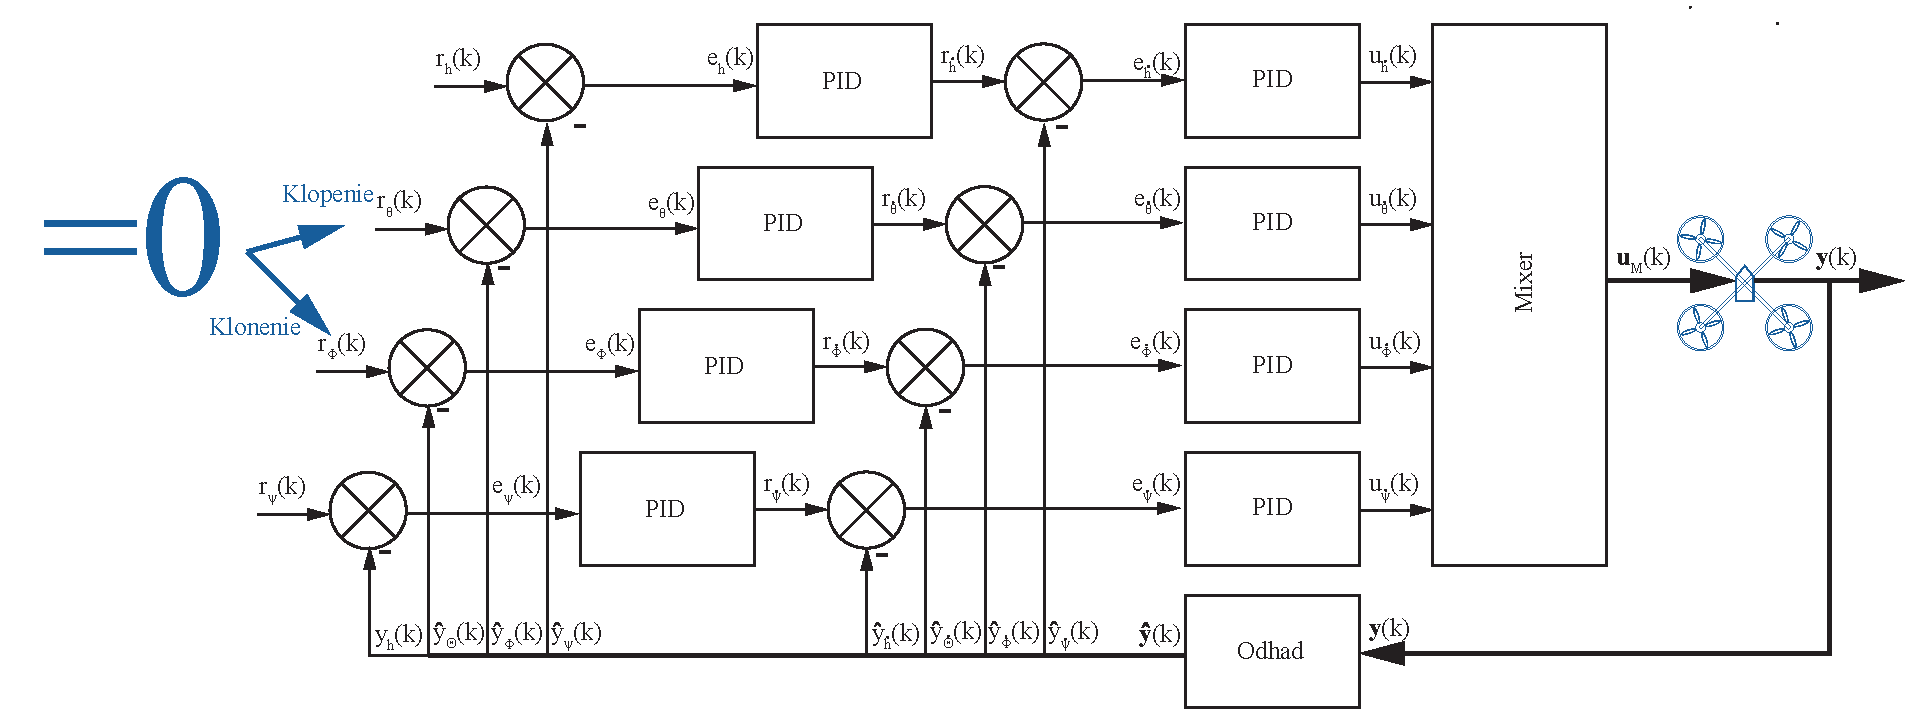
\includegraphics[width=\textwidth]{ATT_Overall2}\\
\end{figure}
  \end{onlyenv}
      \begin{onlyenv}<4>
\begin{figure}
\centering
  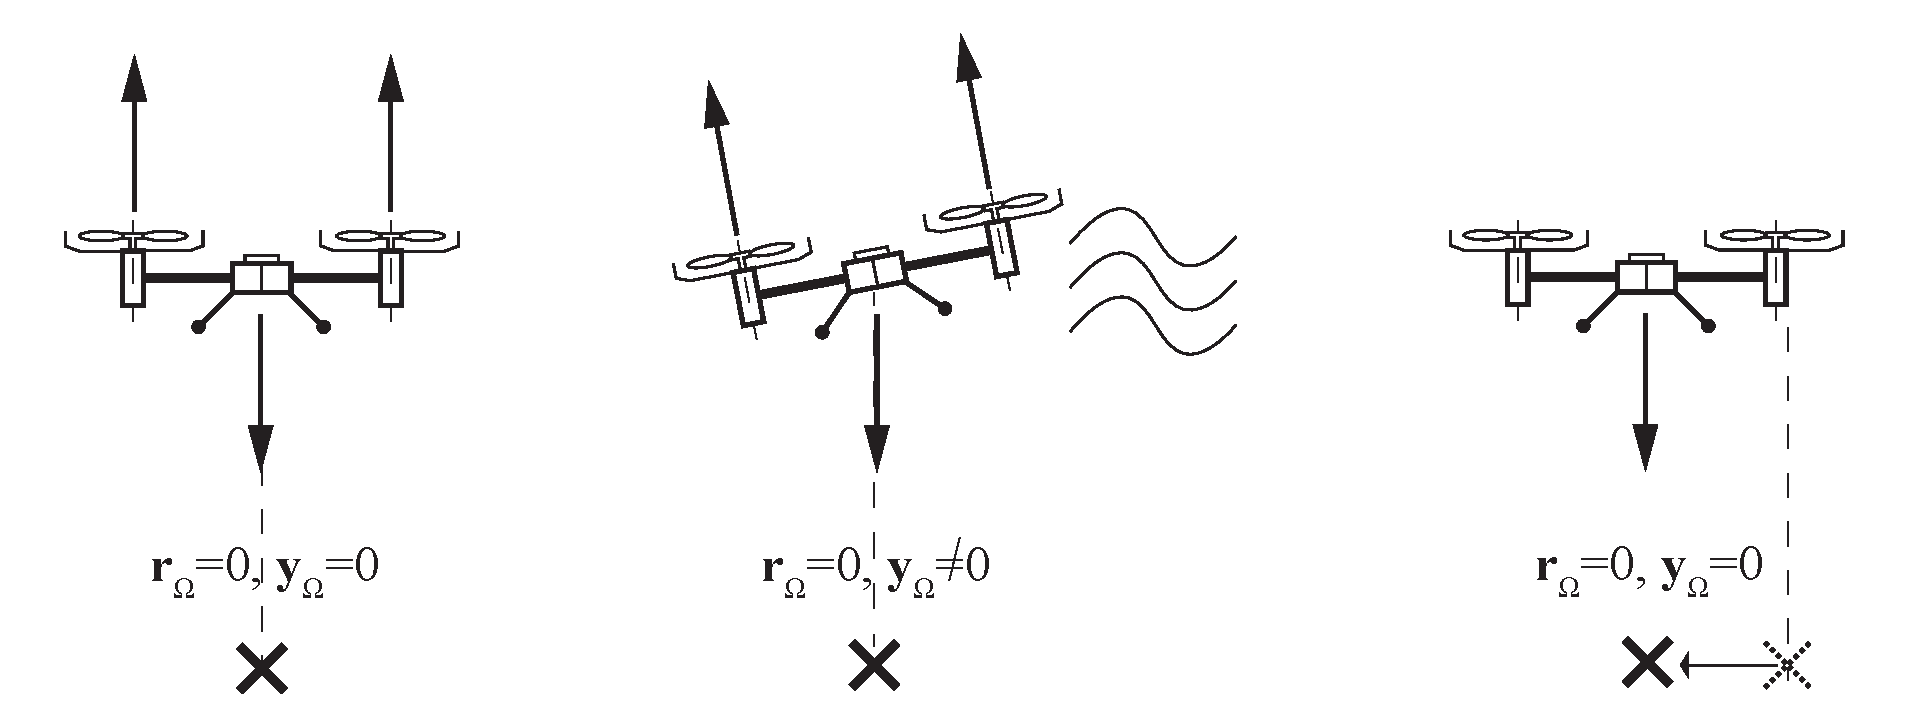
\includegraphics[width=\textwidth]{ATT_Overall3}\\
\end{figure}
  \end{onlyenv}
        \begin{onlyenv}<5>
\begin{figure}
\centering
  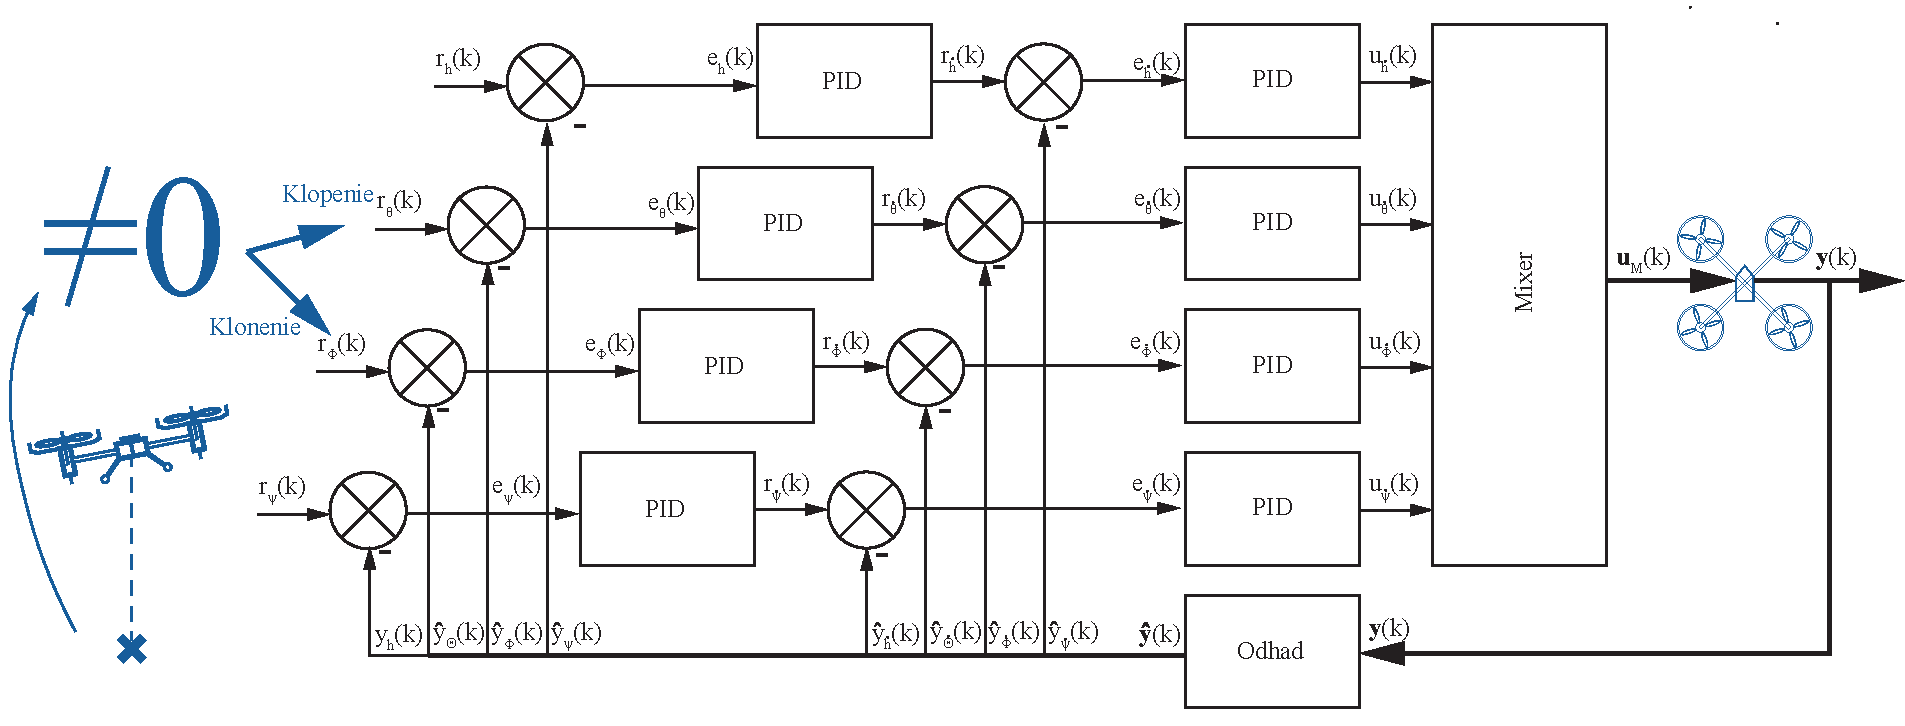
\includegraphics[width=\textwidth]{ATT_Overall4}\\
\end{figure}
  \end{onlyenv}

\end{frame}
